\subsection{Requirements}
The program that we built is a combination of an editor and a simulator: the user is able to construct a conveyor belt system in the editor, after which the movement of luggage in that system can be simulated. Therefore, we have two kinds of requirements: one for the editor part of the program, one for the simulation part of the program.

\subsubsection{Design goals for the editor}
\label{subsubsec:design-goals-editor}
First of all, we want the application to have a very intuitive interface, so that new users can easily find the functionality. Furthermore, we want the interface to be efficient, which means that frequent tasks (for example, building a long, straight conveyor belt) can be executed quickly by the user. Our philosophy is as follows: provide the user with the options to change the program to his/her liking, but provide good default values so that new users are not intimidated by a long list of settings. The settings are ``hidden'' in a clearly labelled submenu so that users who are curious as to what is possible can find it easily and users who are not interested can ignore it easily. Examples of possible settings are changing the position/appearance of the menu bars in the program and changing the mouse sensitivity.

An optional requirement is that we implement some kind of tutorial system that guides the user through their first use of the program. We intend however to make all actions obvious enough, so that such a system is not needed. For example, some programs provide a list of shortcuts in the program. We want to make visible buttons for all actions however, showing the shortcut (if any) in a tooltip when the user hovers the button for a short time.

The single most important requirement on the editor is that placement of blocks is easy, also the placements of multiple blocks that form a line (or more generally, a ``route'') of linked conveyor belts. It must be possible for the user to navigate through the scene in an intuitive way. Also, placing a new block in the scene or selecting a block to build from there or remove it (also refer to Section~\textbf{TO~DO}) should be possible by a simple point-and-select interface. That is, the program should be capable of transforming 2D coordinates of a mouse click into 3D scene coordinates. This transformation will result in a line, so the program must also be able to determine what the user means (clicking the object closest to the user on that line). Details on how we implemented this are given in Section~\textbf{TO~DO}.

Finally, the program should not only be fault-tolerant, but moreover be fault-preventing. For example, if the user tries to place a block on a cell where a block is placed already, then this should be indicated somehow. In no case should the program crash if the user tries to do something that is not possible. We describe in Section~\textbf{TO~DO} how we implemented visual clues in case an impossible situation is (possibly) requested by the user.

\subsubsection{Required functionality for the editor}
\label{subsubsec:req-functionality-simulator}
The program should have support for three types of basic conveyor belts: horizontal belts, sloped belts (ascending \,/\,descending) and bends. (Since we are not modelling a real-world system, this choice is of course somewhat arbitrary; we just chose three simple building blocks with which the user can make useful systems.) Sketches of those three types of belts are given in Figure~\ref{fig:blocks-sketch}.
\begin{figure}
  \begin{center}
    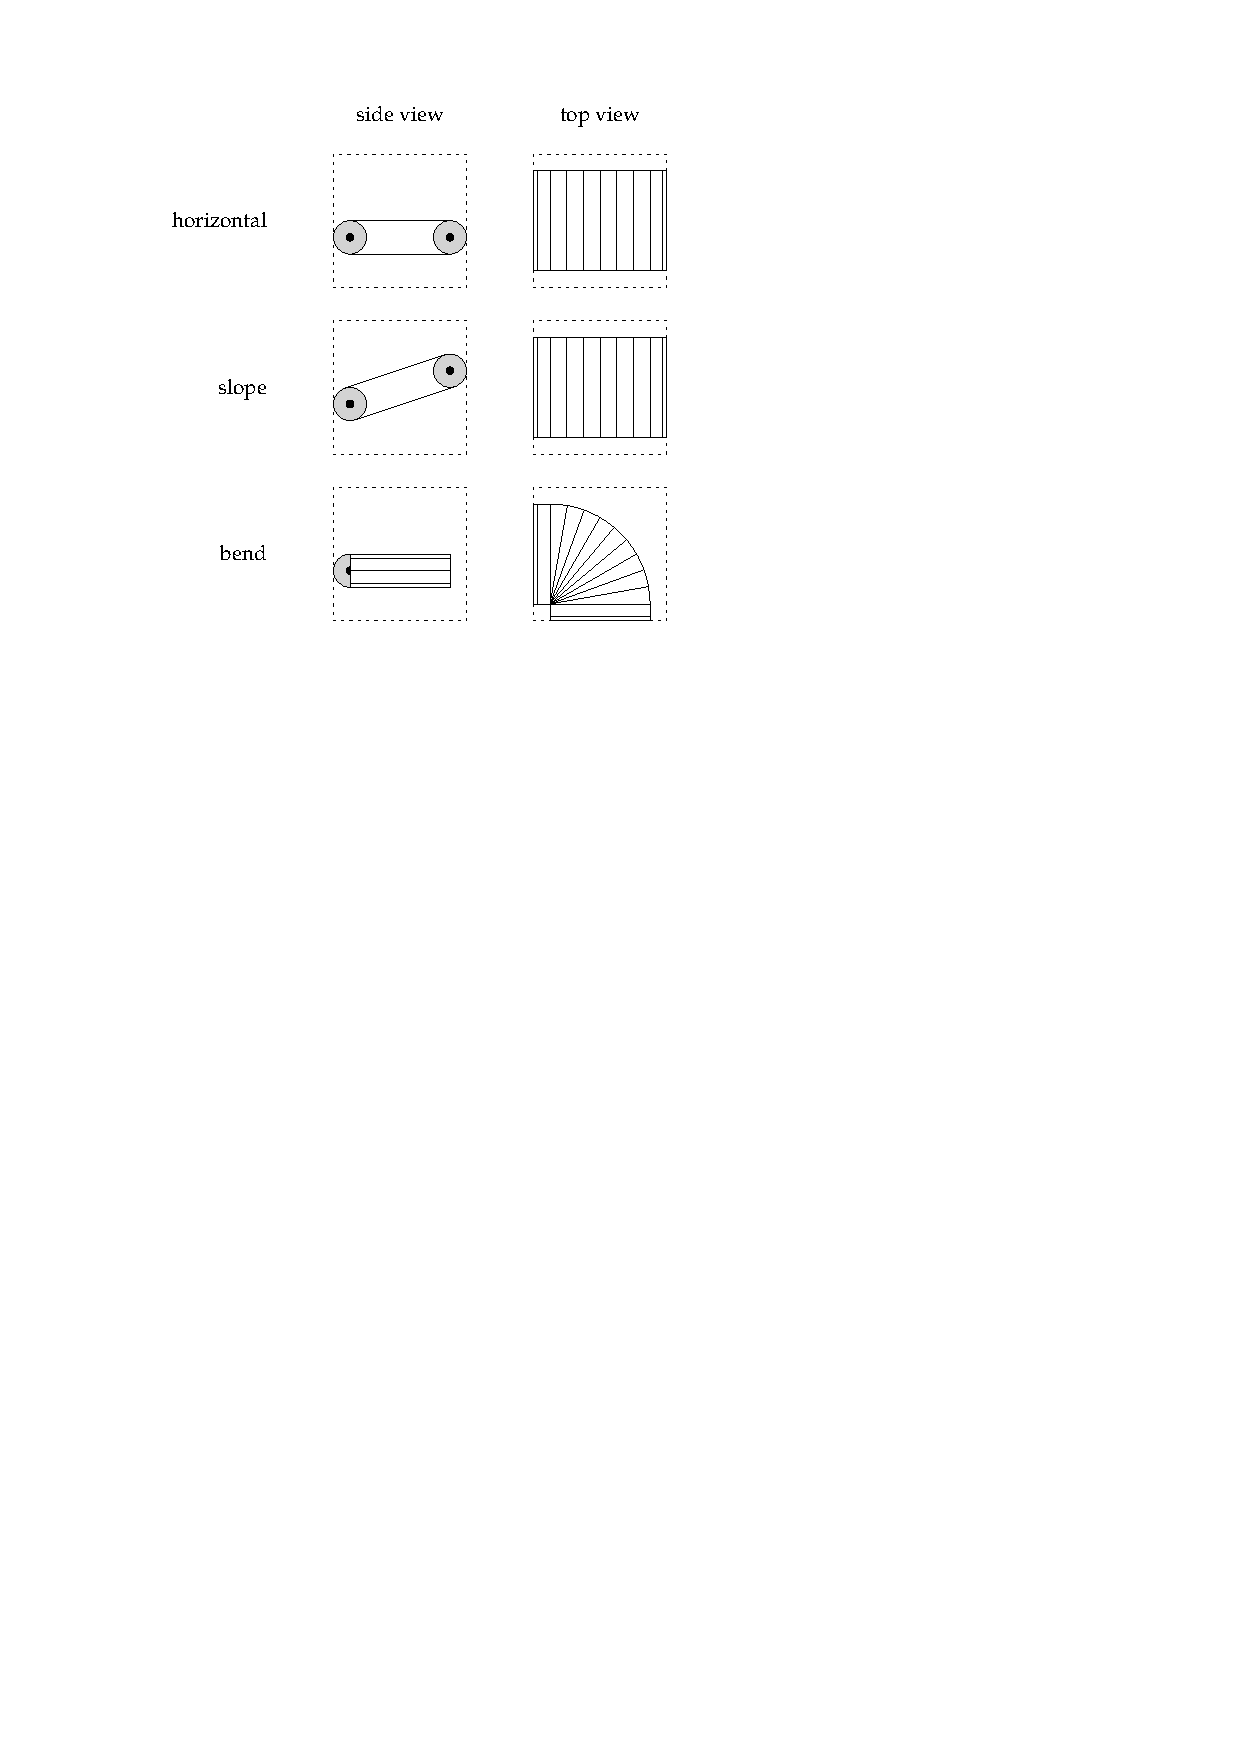
\includegraphics{blocks-sketch}
    \caption{Sketches of the three types of basic conveyor belt blocks available to the user.}
    \label{fig:blocks-sketch}
  \end{center}
\end{figure}

Furthermore, we will add some special blocks to make the system more interesting. First of all, we need an input block that produces luggage, and an output block that the user should move the luggage to. As an optional feature, there could be \emph{scanner} blocks, that scan the type of luggage (as shown by the color of the luggage item) and depending on this type, put the luggage on one of several outgoing conveyor belts. This way, the user can ``sort'' luggage.

\subsubsection{Design goals for the simulator}
\label{subsubsec:design-goals-simulator}
Initially, we did not have a lot of requirements on the simulator. We wanted it to be able to move luggage over the conveyor belts and possibly signal when a piece of luggage would fall on the floor. However, we soon realised that it would be very nice to have collision detection between pieces of luggage. We then decided to switch to using a physics library, giving us the freedom to set more requirements on the simulator. Apart from collision detection between pieces of luggage, we now also wanted realistic collision detection with the conveyor belts. That is, we wanted luggage to precisely follow the bends and rounded corners of the conveyor belts. Furthermore, we were now able to require realistic falling motions when luggage would drop off a conveyor belt. By this we mean that a piece of luggage will usually rotate a bit during its fall, which we did not have at first. Finally, we could have realistic friction when a piece of luggage would fall on/bounce off a conveyor belt.

Some requirements that we had in advance and of course kept when switching to the physics library, are the following. First, the simulation should be fast. By this we mean that calculating the new positions and rotations of objects, et cetera, for one frame should be fast enough to leave enough time for rendering the frame as well. The simulator should also be flexible: it must be easy to add and remove objects, since this is something that happens a lot when the user is editing a conveyor belt system.